\documentclass[11pt,a4paper]{article}
\usepackage[a4paper,left=2.4cm,right=2.4cm,top=2.5cm,bottom=2.5cm]{geometry}
\usepackage{amsmath,amssymb,mathtools}
\usepackage{fontspec}
\usepackage{unicode-math}
\setmainfont{Latin Modern Roman}
\setsansfont{Latin Modern Sans}
\setmonofont{Latin Modern Mono}[Scale=0.88]
\setmathfont{Latin Modern Math}
\usepackage{ragged2e}
\usepackage{booktabs,array,longtable}
\usepackage{enumitem}
\usepackage[dvipsnames]{xcolor}
\usepackage[breakable,skins]{tcolorbox}
\usepackage{fancyhdr}
\usepackage{listings}
\usepackage{tikz}
\usetikzlibrary{arrows.meta,positioning,calc}
\usepackage[hidelinks,pdftitle={Waermeleitung in der einseitig unendlichen Platte},pdfauthor={Claude}]{hyperref}

% ---------- Satz: ohne deutsche Trennmuster -> Flattersatz, keine Trennung ----------
\RaggedRight
\hyphenpenalty=10000
\exhyphenpenalty=10000
\setlength{\parindent}{0pt}
\setlength{\parskip}{0.6em}
\setlength{\emergencystretch}{3em}
\renewcommand{\contentsname}{Inhaltsverzeichnis}
\renewcommand{\figurename}{Abbildung}
\renewcommand{\tablename}{Tabelle}
\numberwithin{equation}{section}
\setlist{itemsep=0.2em,topsep=0.3em}
\setlength{\arraycolsep}{4pt}

\pagestyle{fancy}
\fancyhf{}
\fancyhead[L]{\small Wärmeleitung in der einseitig unendlichen Platte}
\fancyhead[R]{\small\thepage}
\renewcommand{\headrulewidth}{0.3pt}

\lstset{basicstyle=\ttfamily\small,breaklines=true,frame=single,backgroundcolor=\color{gray!6},columns=fullflexible,keepspaces=true}

% ---------- Makros ----------
\newcommand{\dd}{\mathrm{d}}
\newcommand{\pd}[2]{\dfrac{\partial #1}{\partial #2}}
\newcommand{\pdd}[2]{\dfrac{\partial^{2} #1}{\partial #2^{2}}}
\newcommand{\dx}{\Delta x}
\newcommand{\dy}{\Delta y}
\newcommand{\dt}{\Delta t}
\newcommand{\kW}{k_{\mathrm W}}
\newcommand{\thK}{\theta_{K}}
\newcommand{\vthK}{\symbf{\theta}_{K}}
\newcommand{\mA}{\mathbf{A}}
\newcommand{\mB}{\mathbf{B}}
\newcommand{\mE}{\mathbf{E}}
\newcommand{\mC}{\mathbf{C}}
\newcommand{\mI}{\mathbf{I}}
\newcommand{\mG}{\mathbf{G}}
\newcommand{\mGE}{\mathbf{G}_{E}}
\newcommand{\mAd}{\mathbf{A}_{\mathrm d}}
\newcommand{\mBd}{\mathbf{B}_{\mathrm d}}
\newcommand{\mEd}{\mathbf{E}_{\mathrm d}}
\newcommand{\mDx}{\mathbf{D}_{x}}
\newcommand{\mDy}{\mathbf{D}_{y}}
\newcommand{\mPhi}{\symbf{\Phi}}
\newcommand{\vz}{\mathbf{z}}
\newcommand{\vy}{\mathbf{y}}
\newcommand{\vQ}{\mathbf{Q}}
\newcommand{\vr}{\mathbf{r}}
\newcommand{\vv}{\mathbf{v}}
\newcommand{\ve}{\mathbf{e}}
\newcommand{\vone}{\mathbf{1}}
\newcommand{\Rn}{\mathbb{R}}
\newcommand{\Kron}{\otimes}
\newcommand{\norm}[1]{\left\lVert #1\right\rVert}

% ---------- Kästen ----------
\newtcolorbox{ergebnis}[1]{enhanced,breakable,colback=blue!3!white,colframe=blue!55!black,coltitle=white,fonttitle=\bfseries\sffamily,title={#1},left=7pt,right=7pt,top=4pt,bottom=4pt}
\newtcolorbox{hinweis}[1]{enhanced,breakable,colback=orange!6!white,colframe=orange!70!black,coltitle=white,fonttitle=\bfseries\sffamily,title={#1},left=7pt,right=7pt,top=4pt,bottom=4pt}
\newtcolorbox{algo}[1]{enhanced,breakable,colback=green!4!white,colframe=green!40!black,coltitle=white,fonttitle=\bfseries\sffamily,title={#1},left=7pt,right=7pt,top=4pt,bottom=4pt}

\title{\textbf{Wärmeleitung in der einseitig unendlichen Platte}\\[0.4em]
\large Herleitung, Zustandsraummodell, Simulations- und Optimierungsverfahren\\ für die Heizleistung bei vorgegebener Außentemperatur}
\author{}
\date{4.\,Oktober 2026}

\begin{document}
\maketitle
\thispagestyle{fancy}

\renewcommand{\abstractname}{Zusammenfassung}
\begin{abstract}
\noindent
Dieses Dokument leitet ein Rechenmodell für eine Platte her, deren eine Kante eine vorgegebene Temperatur hat (die Außentemperatur) und in der an einer Stelle Wärme zugeführt wird (die Heizleistung $Q$). Ausgegeben wird die Temperatur an einem frei wählbaren Messpunkt. Alle Annahmen, Symbole und Rechenschritte werden einzeln erklärt: von der Energiebilanz über die partielle Differentialgleichung, die Diskretisierung in Ort und Zeit und die Darstellung als lineares Zustandsraummodell bis zur Faltungsdarstellung $\vy = \mPhi\vz_0 + \mGE\vthK + \mG\vQ$. Darauf aufbauend werden Simulationsverfahren, Optimierungsverfahren zur Berechnung einer Heizkurve und der Ablauf der Rechnung (was wird wann berechnet) beschrieben.
\end{abstract}

\tableofcontents
\newpage

% =====================================================================
\section{Aufgabenstellung und Überblick}
% =====================================================================

Betrachtet wird eine dünne, ebene Platte. Ihre eine Kante ($x=0$) hat eine vorgegebene, zeitlich veränderliche Temperatur (die Außentemperatur). In das Innere der Platte wird an einem Punkt Wärme mit der Leistung $Q(t)$ eingebracht. An einem Messpunkt wird die Temperatur $y(t)$ beobachtet.

\begin{center}
\begin{tabular}{lll}
\toprule
 & Größe & Rolle im Modell \\
\midrule
Eingang 1 & $Q(t)$ in W & Heizleistung, \emph{Stellgröße} (wird gewählt bzw. optimiert) \\
Eingang 2 & $\thK(t)$ in K & Kantentemperatur (Außentemperatur), \emph{Störgröße} (ist vorgegeben) \\
Ausgang & $y(t)$ in K & Temperatur am Messpunkt \\
\bottomrule
\end{tabular}
\end{center}

\textbf{Ziel:} Zu einer gegebenen Außentemperaturkurve soll eine Heizkurve $Q(t)$ berechnet werden, die möglichst wenig Leistung verbraucht und dabei die Temperatur $y(t)$ am Messpunkt möglichst konstant hält.

\textbf{Vorgehen} (jeder Schritt ist ein eigener Abschnitt):
\begin{enumerate}
 \item Physik: Energiebilanz und Fouriersches Gesetz $\Rightarrow$ partielle Differentialgleichung (PDGL), Abschnitt~\ref{sec:pdgl}.
 \item Das Gebiet wird in ein Gitter aus Punkten zerlegt, die PDGL wird auf diesen Punkten durch Differenzen ersetzt $\Rightarrow$ gewöhnliches lineares Differentialgleichungssystem $\dot{\vz}=\mA\vz+\mB Q+\mE\thK$, Abschnitt~\ref{sec:ort}.
 \item Zeit in Schritte $\dt$ zerlegen $\Rightarrow$ Rekursion $\vz_{k+1}=\mAd\vz_k+\mBd Q_k+\mEd\thK{}_{,k}$, Abschnitt~\ref{sec:zeit}.
 \item Die Rekursion ausrollen $\Rightarrow$ Faltungsdarstellung $\vy=\dots+\mGE\vthK+\mG\vQ$, Abschnitt~\ref{sec:faltung}.
 \item Klären, was wann berechnet wird, Abschnitt~\ref{sec:wann}. Simulationsverfahren, Abschnitt~\ref{sec:sim}. Optimierungsverfahren, Abschnitt~\ref{sec:opt}.
\end{enumerate}

\begin{hinweis}{Hinweis zur Notation}
In diesem Dokument heißt der Zustandsvektor $\vz$ (in der vorherigen Chat-Antwort $x$). Der Buchstabe $x$ ist hier nur noch die Ortskoordinate. Die Wärmeleitfähigkeit heißt $\kW$ (im Python-Skript \texttt{k}), weil $k$ der Zeitschrittindex ist.
\end{hinweis}

% =====================================================================
\section{Annahmen}
\label{sec:annahmen}
% =====================================================================

Jedes Rechenmodell vereinfacht die Wirklichkeit. Die folgenden Annahmen gelten im gesamten Dokument. Zu jeder steht, was sie bedeutet und wann sie verletzt sein kann.

\begin{description}[style=nextline,leftmargin=1.5em,itemsep=0.5em]
 \item[A1 \;Dünne Platte.] Die Temperatur ist über die Dicke $d$ konstant, hängt also nur von $(x,y,t)$ ab. Das gilt, wenn die Platte dünn gegenüber ihren übrigen Abmessungen ist und gut leitet. Folge: Das Problem ist zweidimensional.
 \item[A2 \;Konstante Materialwerte.] $\kW$, $\rho$, $c$ sind überall in der Platte gleich und hängen weder von Ort noch von Temperatur ab. Folge: Die Gleichung ist \emph{linear}, wodurch die Überlagerung in Abschnitt~\ref{sec:faltung} möglich wird. Bei starker Temperaturabhängigkeit gilt sie nur näherungsweise um einen Arbeitspunkt.
 \item[A3 \;Keine Verluste an Ober- und Unterseite.] Alle Wärme bleibt in der Platte. Eine Erweiterung wäre ein Verlustterm $-\tfrac{2h}{\rho c d}(T-T_\infty)$ mit Wärmeübergangskoeffizient $h$. Er würde in $\mA$ einen Beitrag $-2h/(\rho c d)$ auf der Diagonalen und einen weiteren Eingang erzeugen.
 \item[A4 \;Kante $x=0$: vorgegebene Temperatur.] $T(0,y,t)=T_K(t)$, das heißt idealer thermischer Kontakt zur Außentemperatur. Ist die Kopplung nicht ideal, ersetzt man diese Bedingung durch eine Wärmeübergangsbedingung (Robin-Bedingung). Die Struktur der Herleitung bleibt gleich.
 \item[A5 \;Fernrand $x=L_x$: ungestörte Temperatur.] $T(L_x,y,t)=T_0$. Das ersetzt die „unendliche“ Platte. Es ist eine Abschneidung, die nur gilt, solange die Wärme den Fernrand nicht erreicht. Faustregel: $L_x$ deutlich größer als die Eindringtiefe $\delta(t)\approx 4\sqrt{\alpha t}$ (Begründung in Abschnitt~\ref{sec:analytisch}).
 \item[A6 \;Seitenränder $y=0$ und $y=L_y$: wärmeisoliert.] Kein Wärmestrom durch diese Ränder. Auch das ist eine Abschneidung und gilt, solange Quelle und Messpunkt weiter vom Rand entfernt sind als $\delta(t)$.
 \item[A7 \;Punktquelle.] Die Heizleistung $Q$ wird in einem einzigen Gitterpunkt (genauer: einer Gitterzelle) eingebracht.
 \item[A8 \;Anfangszustand.] Zum Zeitpunkt $t=0$ hat die Platte überall die Temperatur $T_0$. Anderenfalls kommt in Abschnitt~\ref{sec:faltung} ein Anfangswertterm hinzu.
 \item[A9 \;Stückweise konstante Eingänge.] Innerhalb eines Zeitschritts sind $Q$ und $\thK$ konstant (Halteglied nullter Ordnung, englisch \emph{zero-order hold}, ZOH).
 \item[A10 \;Ideale Messung und ideales Stellglied.] Der Messwert ist die exakte Gitterpunkttemperatur, und die Heizleistung wirkt ohne Verzögerung durch das Heizelement selbst.
\end{description}

% =====================================================================
\section{Symbole und Einheiten}
% =====================================================================

\begin{longtable}{@{}>{\RaggedRight}p{2.4cm}>{\RaggedRight}p{6.4cm}>{\RaggedRight}p{1.9cm}>{\RaggedRight}p{3.2cm}@{}}
\toprule
Symbol & Bedeutung & Einheit & Herkunft \\
\midrule
\endhead
$\kW$ & Wärmeleitfähigkeit & W/(m\,K) & Materialtabelle \\
$\rho$ & Dichte & kg/m$^3$ & Materialtabelle \\
$c$ & spezifische Wärmekapazität & J/(kg\,K) & Materialtabelle \\
$d$ & Plattendicke & m & Geometrie \\
$\alpha=\kW/(\rho c)$ & Temperaturleitfähigkeit & m$^2$/s & berechnet \\
$L_x, L_y$ & Abmessungen des betrachteten Gebiets & m & gewählt \\
$\dx,\dy$ & Abstand benachbarter Gitterpunkte & m & gewählt \\
$\dt$ & Zeitschritt & s & gewählt \\
$T$ & Temperatur & K bzw.\ °C & Messgröße \\
$T_0$ & Anfangs- und Fernfeldtemperatur & °C & gegeben \\
$\theta=T-T_0$ & Temperaturerhöhung gegenüber $T_0$ & K & Definition \\
$\thK(t)$ & Erhöhung der Kantentemperatur, $\thK=T_K-T_0$ & K & Außentemperatur \\
$Q(t)$ & Heizleistung & W & Eingang \\
$(x_S,y_S)$ & Ort der Heizquelle & m & gewählt \\
$(x_M,y_M)$ & Ort des Messpunkts & m & gewählt \\
$y(t)$ & Temperaturerhöhung am Messpunkt & K & Ausgang \\
$m,\;p$ & Anzahl unbekannter Gitterpunkte in $x$- bzw.\ $y$-Richtung & --- & $m=n_x-2$, $p=n_y$ \\
$n=m\,p$ & Anzahl aller Unbekannten (Zustände) & --- & berechnet \\
$i,\;j$ & Gitterindizes in $x$- bzw.\ $y$-Richtung & --- & --- \\
$a=\alpha/\dx^2$ & Kopplung zu den Nachbarn in $x$ & 1/s & berechnet \\
$b=\alpha/\dy^2$ & Kopplung zu den Nachbarn in $y$ & 1/s & berechnet \\
$s=2a+2b$ & Betrag der Diagonale von $\mA$ & 1/s & berechnet \\
$\beta=\dfrac{1}{\rho c\,d\,\dx\,\dy}$ & Umrechnung Leistung $\to$ Erwärmungsrate & K/(s\,W) & Abschnitt~\ref{sec:pdgl} \\
$\vz(t)\in\Rn^n$ & Zustandsvektor: alle $\theta_{i,j}$ als Liste & K & Abschnitt~\ref{sec:ort} \\
$\mA,\mB,\mE,\mC$ & Matrizen des zeitkontinuierlichen Modells & --- & Abschnitt~\ref{sec:ort} \\
$\mAd,\mBd,\mEd$ & Matrizen des zeitdiskreten Modells & --- & Abschnitt~\ref{sec:zeit} \\
$k,\;q$ & Zeitschrittindizes, $t_k=k\,\dt$ & --- & --- \\
$\ell$ & Verzögerung in Zeitschritten (Index der Impulsantwort) & --- & --- \\
$h_\ell,\;h^E_\ell$ & Impulsantwort von $Q$ bzw.\ $\thK$ zum Messpunkt & K/W bzw.\ K/K & Abschnitt~\ref{sec:faltung} \\
$\mG,\;\mGE$ & untere Dreiecks-Toeplitz-Matrizen aus $h_\ell$ bzw.\ $h^E_\ell$ & wie $h$ & Abschnitt~\ref{sec:faltung} \\
$\mPhi$ & Antwort des Anfangszustands & --- & Abschnitt~\ref{sec:faltung} \\
$N$ & Horizontlänge (Zahl der Zeitschritte) & --- & gewählt \\
$y_\mathrm{ref}$ & Soll-Temperaturerhöhung am Messpunkt & K & Vorgabe \\
$\lambda$ & Regularisierungsgewicht (Strafe auf Heizleistung) & K$^2$/W$^2$ & gewählt \\
\bottomrule
\end{longtable}

Wir rechnen mit der \emph{Temperaturerhöhung} $\theta=T-T_0$ statt mit $T$. Die PDGL enthält nur Ableitungen von $T$, und die Konstante $T_0$ fällt bei Ableitungen weg. Deshalb erfüllt $\theta$ dieselbe Gleichung. Der Vorteil: Anfangswert und Fernrand sind dann einfach $0$. Am Ende rechnet man mit $T=T_0+\theta$ zurück.

% =====================================================================
\section{Physikalische Grundlagen und die Wärmeleitungsgleichung}
\label{sec:pdgl}
% =====================================================================

\subsection{Begriffe}

\textbf{Innere Energie und Wärmekapazität.} Erwärmt man einen Körper der Masse $m_K$ um $\Delta T$, nimmt er die Energie
\begin{equation}
 \Delta U = m_K\,c\,\Delta T
\end{equation}
auf. $c$ ist die spezifische Wärmekapazität in J/(kg\,K).

\textbf{Wärmestrom.} Der Wärmestrom $\Phi$ (in W $=$ J/s) ist die pro Sekunde fließende Energie. Die Wärmestromdichte $q_x$ (in W/m$^2$) ist der Wärmestrom pro Fläche in $x$-Richtung.

\textbf{Fouriersches Gesetz.} Wärme fließt von warm nach kalt, und zwar proportional zum Temperaturgefälle:
\begin{equation}
 q_x=-\kW\,\pd{T}{x},\qquad q_y=-\kW\,\pd{T}{y}.
\end{equation}
Das Minuszeichen sorgt dafür, dass $q_x>0$ ist, wenn die Temperatur mit $x$ abnimmt (Wärme fließt dann in $+x$-Richtung).

\subsection{Energiebilanz an einem kleinen Plattenelement}

Wir betrachten ein Element mit den Kantenlängen $\dd x$ und $\dd y$ und der Dicke $d$. Seine Masse ist $\rho\,d\,\dd x\,\dd y$, seine innere Energie also
\begin{equation}
 U = \rho\,c\,d\,\dd x\,\dd y\;T.
\end{equation}
Energieerhaltung bedeutet: Die Änderung der gespeicherten Energie pro Sekunde ist gleich zufließender minus abfließender Wärmestrom plus Heizleistung im Element:
\begin{equation}
 \pd{U}{t}=\Phi_\mathrm{ein}-\Phi_\mathrm{aus}+P_\mathrm{Quelle}.
\end{equation}

\textbf{Wärmestrom in $x$-Richtung.} Durch die linke Seitenfläche (Fläche $d\,\dd y$) tritt $q_x(x)\,d\,\dd y$ ein, durch die rechte Seitenfläche tritt $q_x(x+\dd x)\,d\,\dd y$ aus. Mit der Taylor-Entwicklung $q_x(x+\dd x)\approx q_x(x)+\pd{q_x}{x}\dd x$ ist der Nettozufluss
\begin{equation}
 \Phi_{x,\mathrm{ein}}-\Phi_{x,\mathrm{aus}}
 = -\pd{q_x}{x}\,\dd x\,d\,\dd y
 = \kW\,\pdd{T}{x}\,\dd x\,\dd y\,d .
\end{equation}
Das zweite Gleichheitszeichen folgt aus dem Fourierschen Gesetz: $-\pd{q_x}{x}=\kW\pdd{T}{x}$. In $y$-Richtung gilt dasselbe mit vertauschten Rollen.

\textbf{Gesamtbilanz.} Einsetzen und Teilen durch $\rho\,c\,d\,\dd x\,\dd y$ ergibt mit $\alpha=\kW/(\rho c)$:
\begin{equation}
 \pd{T}{t}=\alpha\left(\pdd{T}{x}+\pdd{T}{y}\right)+\frac{P_\mathrm{Quelle}}{\rho\,c\,d\,\dd x\,\dd y}.
 \label{eq:pdgl_roh}
\end{equation}
Das ist die \emph{Wärmeleitungsgleichung} mit Quellterm. $\alpha$ heißt Temperaturleitfähigkeit. Je größer $\alpha$, desto schneller gleichen sich Temperaturunterschiede aus. Für Aluminium ($\kW=200$, $\rho=2700$, $c=900$) ist $\alpha\approx 8{,}2\cdot10^{-5}$\,m$^2$/s.

\subsection{Quellterm: Punktquelle}

Eine Punktquelle der Leistung $Q$ am Ort $(x_S,y_S)$ schreibt man mit der Delta-Distribution $\delta$ als Leistungsdichte (Leistung pro Fläche, W/m$^2$) $Q\,\delta(x-x_S)\,\delta(y-y_S)$. Dabei ist $\delta$ so definiert, dass das Integral über eine Umgebung des Punktes $1$ ergibt. Pro Sekunde zugeführte Energie ist dann gerade $Q$. Für die Gleichung teilt man noch durch $\rho c d$, weil die Plattendicke $d$ schon in der Bilanz steckt:

\begin{ergebnis}{PDGL mit Anfangs- und Randbedingungen (in $\theta=T-T_0$)}
\begin{align}
 \pd{\theta}{t} &= \alpha\left(\pdd{\theta}{x}+\pdd{\theta}{y}\right)+\frac{Q(t)}{\rho\,c\,d}\;\delta(x-x_S)\,\delta(y-y_S), \label{eq:pdgl}\\[0.3em]
 \theta(x,y,0) &= 0 && \text{(Anfangsbedingung, A8)}\notag\\
 \theta(0,y,t) &= \thK(t) && \text{(Kante, A4)}\notag\\
 \theta(L_x,y,t) &= 0 && \text{(Fernrand, A5)}\notag\\
 \pd{\theta}{y}(x,0,t) &= \pd{\theta}{y}(x,L_y,t)=0 && \text{(isolierte Seitenränder, A6)}\notag
\end{align}
\end{ergebnis}

\subsection{Eine Randbedingung pro Randstück}

Die Gleichung ist in jeder Raumrichtung von zweiter Ordnung. Damit die Lösung eindeutig ist, braucht man auf jedem Randstück \emph{genau eine} Bedingung: entweder die Temperatur ist vorgegeben (Dirichlet), oder der Wärmestrom ist vorgegeben (Neumann), oder eine Kombination (Robin). Zwei Bedingungen auf demselben Randstück sind überbestimmt, keine Bedingung ist unterbestimmt. Dazu kommt eine Anfangsbedingung, weil die Gleichung in der Zeit von erster Ordnung ist.

Die Heizquelle ist \emph{keine} Randbedingung. Sie liegt im Inneren und steht als Summand rechts in der Gleichung selbst. Die Gleichung gilt auch im Quellpunkt, und die Lösung entscheidet selbst, welche Temperatur sich dort einstellt.

% =====================================================================
\section{Räumliche Diskretisierung}
\label{sec:ort}
% =====================================================================

Ein Computer kann keine Funktion $\theta(x,y,t)$ auf unendlich vielen Punkten verwalten. Wir legen deshalb ein Gitter über die Platte und verfolgen nur die Temperaturen auf den Gitterpunkten. Die Ableitungen nach dem Ort ersetzen wir durch Differenzen. Die Zeit bleibt vorerst kontinuierlich („Linienmethode“).

\subsection{Ersatz der zweiten Ableitung durch eine Differenz}

Für eine glatte Funktion $T$ gilt die Taylor-Entwicklung mit Schrittweite $h$:
\begin{align}
 T(x+h)&=T(x)+h\,T'(x)+\tfrac{h^2}{2}T''(x)+\tfrac{h^3}{6}T'''(x)+\tfrac{h^4}{24}T''''(x)+\dots\\
 T(x-h)&=T(x)-h\,T'(x)+\tfrac{h^2}{2}T''(x)-\tfrac{h^3}{6}T'''(x)+\tfrac{h^4}{24}T''''(x)-\dots
\end{align}
Addiert man beide Zeilen, heben sich alle ungeraden Terme auf:
\begin{equation}
 T(x+h)+T(x-h)=2\,T(x)+h^2\,T''(x)+\tfrac{h^4}{12}T''''(x)+\dots
\end{equation}
Umgestellt nach $T''$:
\begin{equation}
 \boxed{\;T''(x)\approx\frac{T(x+h)-2\,T(x)+T(x-h)}{h^2}\;}
 \qquad\text{(Fehler von der Größenordnung } h^2\text{)}.
 \label{eq:zweitediff}
\end{equation}
In Worten: Die zweite Ableitung ist (linker Nachbar $-\,2\cdot$ Mitte $+$ rechter Nachbar), geteilt durch den Abstand zum Quadrat. Sie misst, wie stark ein Punkt vom Mittelwert seiner Nachbarn abweicht.

\subsection{Gitter, Unbekannte und Nummerierung}

Die Gitterpunkte liegen bei $x_i=i\,\dx$ mit $i=0,\dots,m+1$ und bei $y_j=j\,\dy$ mit $j=0,\dots,p-1$. Die Nachbarpunkte in $x$-Richtung heißen $i\pm1$.
\begin{itemize}
 \item $i=0$ ist die Kante (Temperatur $\thK(t)$ ist \emph{bekannt}, kein Zustand).
 \item $i=m+1$ ist der Fernrand (Temperatur $0$ ist \emph{bekannt}, kein Zustand).
 \item \textbf{Unbekannt} sind $\theta_{i,j}(t)$ für $i=1,\dots,m$ und $j=0,\dots,p-1$, also $n=m\,p$ Zustände. Die Punkte $j=0$ und $j=p-1$ liegen auf den isolierten Rändern und sind ebenfalls Unbekannte.
\end{itemize}
Alle Unbekannten werden zu einer Liste, dem \emph{Zustandsvektor} $\vz(t)\in\Rn^n$, zusammengefasst. Die Reihenfolge ist: erst alle $j$ für $i=1$, dann alle $j$ für $i=2$, usw.:
\begin{equation}
 \vz=\bigl(\theta_{1,0},\dots,\theta_{1,p-1},\;\theta_{2,0},\dots,\theta_{2,p-1},\;\dots,\;\theta_{m,0},\dots,\theta_{m,p-1}\bigr)^{\!\top}.
\end{equation}
Der Punkt $(i,j)$ steht also an Position $\kappa(i,j)=(i-1)\,p+j+1$ der Liste (Zählung ab 1).

\begin{figure}[ht]
\centering
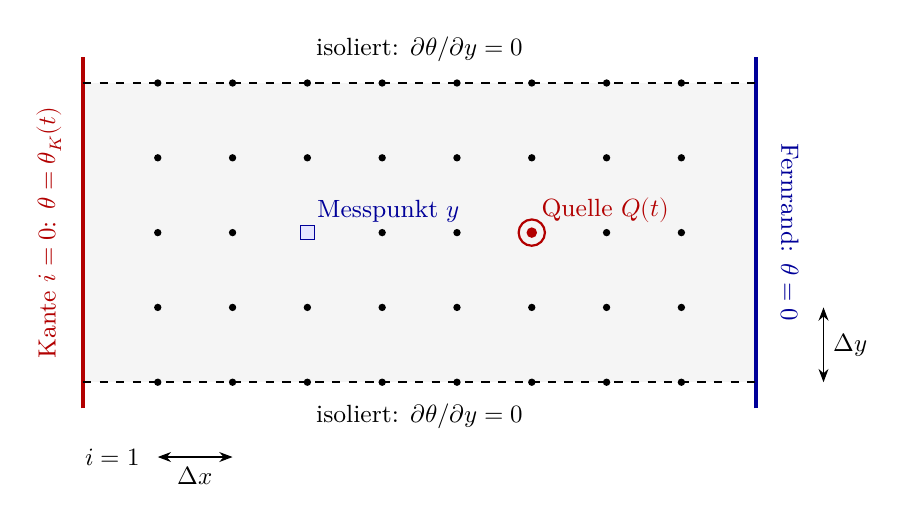
\begin{tikzpicture}[scale=0.95,>=Stealth]
 \fill[gray!8] (0,0) rectangle (9,4);
 \foreach \i in {1,...,8}{\foreach \j in {0,...,4}{\fill (\i,\j) circle (1.4pt);}}
 \draw[red!70!black,line width=1.6pt] (0,-0.35) -- (0,4.35);
 \draw[blue!60!black,line width=1.6pt] (9,-0.35) -- (9,4.35);
 \draw[dashed,thick] (0,0) -- (9,0);
 \draw[dashed,thick] (0,4) -- (9,4);
 \draw[red!70!black,thick] (6,2) circle (5pt);
 \fill[red!70!black] (6,2) circle (2pt);
 \node[red!70!black,above right] at (6,2) {\small Quelle $Q(t)$};
 \node[draw,blue!60!black,fill=blue!10,inner sep=2.5pt] at (3,2) {};
 \node[blue!60!black,above right] at (3,2) {\small Messpunkt $y$};
 \node[red!70!black,rotate=90] at (-0.45,2) {\small Kante $i=0$: $\theta=\thK(t)$};
 \node[blue!60!black,rotate=-90] at (9.45,2) {\small Fernrand: $\theta=0$};
 \node at (4.5,4.45) {\small isoliert: $\partial\theta/\partial y=0$};
 \node at (4.5,-0.45) {\small isoliert: $\partial\theta/\partial y=0$};
 \draw[<->] (1,-1.0) -- (2,-1.0) node[midway,below] {\small $\dx$};
 \draw[<->] (9.9,0) -- (9.9,1) node[midway,right] {\small $\dy$};
 \node at (1,-1.0) [left=3pt] {\small $i=1$};
\end{tikzpicture}
\caption{Gitter der Platte. Die schwarzen Punkte sind die Unbekannten (Zustände). Kante und Fernrand sind vorgegeben und selbst keine Unbekannten. Die Punkte auf den gestrichelten Rändern gehören zu den Unbekannten, ihre Gleichung enthält die Isolierbedingung.}
\end{figure}

\subsection{Die Gleichung für einen einzelnen Gitterpunkt}

Ersetzt man in~\eqref{eq:pdgl} beide zweiten Ableitungen durch~\eqref{eq:zweitediff}, ergibt sich für einen Punkt, dessen vier Nachbarn alle Unbekannte sind:
\begin{equation}
 \dot\theta_{i,j}=\underbrace{\tfrac{\alpha}{\dx^2}}_{a}\bigl(\theta_{i+1,j}-2\theta_{i,j}+\theta_{i-1,j}\bigr)
 +\underbrace{\tfrac{\alpha}{\dy^2}}_{b}\bigl(\theta_{i,j+1}-2\theta_{i,j}+\theta_{i,j-1}\bigr).
 \label{eq:knoten}
\end{equation}
Der Punkt über $\theta$ bedeutet die Ableitung nach der Zeit. Die Zahlen $a$ und $b$ geben an, wie stark ein Punkt an seine Nachbarn in $x$- bzw.\ $y$-Richtung gekoppelt ist (Einheit 1/s).

\textbf{Randfälle:}
\begin{enumerate}
 \item \emph{Nachbar ist die Kante} ($i=1$): $\theta_{0,j}=\thK(t)$ ist bekannt. Der Term $a\,\thK(t)$ bleibt als Summand stehen, er ist ein \emph{Eingang} (daraus entsteht der Vektor $\mE$).
 \item \emph{Nachbar ist der Fernrand} ($i=m$): $\theta_{m+1,j}=0$, der Term entfällt.
 \item \emph{Isolierter Rand} ($j=0$ bzw.\ $j=p-1$): Keine Wärme fließt durch den Rand, also $\pd{\theta}{y}=0$. Wir denken uns einen Hilfspunkt (\emph{Geisterpunkt}) $\theta_{i,-1}$ außerhalb und setzen ihn gleich dem inneren Nachbarn: $\theta_{i,-1}=\theta_{i,1}$. Die Zentraldifferenz $\bigl(\theta_{i,1}-\theta_{i,-1}\bigr)/(2\dy)$ ist dann $0$ (und sie approximiert $\pd{\theta}{y}$ mit einem Fehler der Ordnung $\dy^2$). Der $y$-Term in~\eqref{eq:knoten} wird zu
 \begin{equation}
  b\bigl(\theta_{i,1}-2\theta_{i,0}+\theta_{i,-1}\bigr)=2\,b\,\bigl(\theta_{i,1}-\theta_{i,0}\bigr).
 \end{equation}
 Analog am Rand $j=p-1$.
 \item \emph{Quellpunkt} $(i_S,j_S)$: Das Gitterelement um den Punkt hat die Fläche $\dx\,\dy$. Die Delta-Distribution wird dort durch ihren Mittelwert $1/(\dx\,\dy)$ ersetzt (ihr Integral über die Zelle muss $1$ sein). Es kommt der Summand
 \begin{equation}
  \beta\,Q(t),\qquad \beta=\frac{1}{\rho\,c\,d\,\dx\,\dy}\quad\Bigl[\tfrac{\mathrm K}{\mathrm s\,\mathrm W}\Bigr]
 \end{equation}
 hinzu. Einheitenprüfung: W\,/\,(kg/m$^3\cdot$J/(kg\,K)$\cdot$m$^3$) $=$ W\,/\,(J/K) $=$ K/s. Der Quellpunkt sollte mindestens einen Gitterpunkt vom Rand entfernt liegen.
\end{enumerate}

\subsection{Beispiel in einer Dimension}

Ein Stab mit drei Unbekannten $\theta_1,\theta_2,\theta_3$, links die Kante, rechts der Fernrand:
\begin{center}
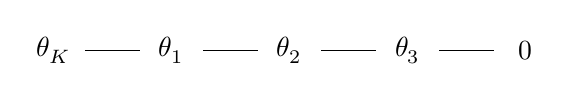
\begin{tikzpicture}
 \node at (0,0) {$\thK$}; \node at (1.5,0) {$\theta_1$}; \node at (3,0) {$\theta_2$}; \node at (4.5,0) {$\theta_3$}; \node at (6,0) {$0$};
 \draw (0.4,0) -- (1.1,0); \draw (1.9,0) -- (2.6,0); \draw (3.4,0) -- (4.1,0); \draw (4.9,0) -- (5.6,0);
\end{tikzpicture}
\end{center}
Mit $a=\alpha/\dx^2$ lauten die drei Gleichungen
\begin{align*}
 \dot\theta_1&=a\,(\thK-2\theta_1+\theta_2),\\
 \dot\theta_2&=a\,(\theta_1-2\theta_2+\theta_3),\\
 \dot\theta_3&=a\,(\theta_2-2\theta_3+0).
\end{align*}
Als Matrixgleichung (die Matrix mal den Vektor ergibt zeilenweise genau die drei Gleichungen):
\begin{equation*}
 \begin{pmatrix}\dot\theta_1\\\dot\theta_2\\\dot\theta_3\end{pmatrix}
 = a\begin{pmatrix}-2&1&0\\1&-2&1\\0&1&-2\end{pmatrix}
 \begin{pmatrix}\theta_1\\\theta_2\\\theta_3\end{pmatrix}
 + a\begin{pmatrix}1\\0\\0\end{pmatrix}\thK .
\end{equation*}
Der Vektor $a\,(1,0,0)^\top$ vor $\thK$ ist das, was später $\mE$ heißt: Nur der Punkt neben der Kante spürt $\thK$ direkt.

\subsection{Beispiel in zwei Dimensionen (sechs Unbekannte)}

Die Unbekannten liegen in der Reihenfolge
$\vz=(\theta_{1,0},\theta_{1,1},\theta_{1,2},\theta_{2,0},\theta_{2,1},\theta_{2,2})^\top$. Mit $s=2a+2b$ lauten z.\,B.\ die Gleichungen
\begin{align*}
 \dot\theta_{1,1}&=a(\thK-2\theta_{1,1}+\theta_{2,1})+b(\theta_{1,0}-2\theta_{1,1}+\theta_{1,2}),\\
 \dot\theta_{1,0}&=a(\thK-2\theta_{1,0}+\theta_{2,0})+2b(\theta_{1,1}-\theta_{1,0}).
\end{align*}
Schreibt man alle sechs Gleichungen untereinander, entsteht
\begin{equation}
 \mA=\begin{pmatrix}
 -s&2b&0&a&0&0\\
 b&-s&b&0&a&0\\
 0&2b&-s&0&0&a\\
 a&0&0&-s&2b&0\\
 0&a&0&b&-s&b\\
 0&0&a&0&2b&-s
 \end{pmatrix},\quad
 \mE=\begin{pmatrix}a\\a\\a\\0\\0\\0\end{pmatrix}.
 \label{eq:A6}
\end{equation}
Die Diagonale ist $-s=-(2a+2b)$. Ein Eintrag $a$ steht dort, wo der Nachbar in $x$-Richtung liegt, ein Eintrag $b$ bei einem Nachbarn in $y$-Richtung, und $2b$ beim inneren Nachbarn eines Randpunkts (aus der Geisterpunkt-Spiegelung). Liegt die Quelle im Punkt $(2,1)$ und der Messpunkt im Punkt $(1,1)$, dann ist
\begin{equation}
 \mB=\beta\,(0,0,0,0,1,0)^\top,\qquad \mC=(0,1,0,0,0,0).
\end{equation}

\subsection{Allgemeine Form über das Kronecker-Produkt}

Für beliebige $m$ und $p$ baut man dieselbe Matrix aus zwei kleinen Bausteinen. Die eindimensionalen Operatoren sind
\begin{equation}
 \mDx=\frac{1}{\dx^2}
 \begin{pmatrix}-2&1&&\\1&-2&1&\\&\ddots&\ddots&\ddots\\&&1&-2\end{pmatrix}\in\Rn^{m\times m},\qquad
 \mDy=\frac{1}{\dy^2}
 \begin{pmatrix}-2&2&&\\1&-2&1&\\&\ddots&\ddots&\ddots\\&&2&-2\end{pmatrix}\in\Rn^{p\times p}.
\end{equation}
Die $2$ in der ersten und letzten Zeile von $\mDy$ stammt aus der Geisterpunkt-Spiegelung. Das \emph{Kronecker-Produkt} zweier Matrizen $\mathbf{M}\in\Rn^{m\times m}$ und $\mathbf{N}\in\Rn^{p\times p}$ ist die Blockmatrix
\begin{equation}
 \mathbf{M}\Kron\mathbf{N}=\begin{pmatrix}M_{11}\mathbf{N}&\cdots&M_{1m}\mathbf{N}\\\vdots&&\vdots\\M_{m1}\mathbf{N}&\cdots&M_{mm}\mathbf{N}\end{pmatrix}\in\Rn^{mp\times mp}.
\end{equation}
Bei der Nummerierung $\kappa=(i-1)p+j+1$ wirkt $\mDx\Kron\mI_p$ auf die Nachbarn in $x$-Richtung (Listenabstand $p$) und $\mI_m\Kron\mDy$ auf die Nachbarn in $y$-Richtung (Listenabstand $1$ innerhalb eines Blocks). Daraus folgt
\begin{ergebnis}{Systemmatrix und Vektoren}
\begin{align}
 \mA&=\alpha\bigl(\mDx\Kron\mI_p+\mI_m\Kron\mDy\bigr)\in\Rn^{n\times n},\\
 \mE&=\frac{\alpha}{\dx^2}\,\bigl(\ve_1^{(m)}\Kron\vone_p\bigr)\in\Rn^{n},\\
 \mB&=\beta\;\ve_{\kappa(i_S,j_S)}\in\Rn^{n},\qquad \beta=\frac{1}{\rho c d\,\dx\,\dy},\\
 \mC&=\ve_{\kappa(i_M,j_M)}^{\top}\in\Rn^{1\times n}.
\end{align}
Dabei ist $\ve_r$ der Einheitsvektor mit einer $1$ an Position $r$ und $\vone_p$ der Vektor aus lauter Einsen der Länge $p$.
\end{ergebnis}
In Blockform hat $\mA$ in den Diagonalblöcken $\alpha\bigl(\mDy-\tfrac{2}{\dx^2}\mI_p\bigr)$ und in den beiden Nebendiagonalen $\tfrac{\alpha}{\dx^2}\mI_p$. Für $m=2$, $p=3$ ergibt das genau die Matrix aus~\eqref{eq:A6}. Liegt der Messpunkt zwischen Gitterpunkten, wählt man in $\mC$ die Nachbarpunkte mit Gewichten, die sich zu $1$ summieren (bilineare Interpolation).

\subsection{Eigenschaften der Systemmatrix}

\begin{enumerate}
 \item \textbf{Dünn besetzt:} Jede Zeile hat höchstens fünf Einträge ungleich null. Bei großen Gittern speichert man $\mA$ daher als Sparse-Matrix.
 \item \textbf{Reelle Eigenwerte:} $\mDy=\symbf{\Lambda}\mathbf{S}\symbf{\Lambda}^{-1}$ mit der symmetrischen Matrix $\mathbf{S}$ (Einträge $\sqrt2/\dy^2$ statt $2/\dy^2$ bzw.\ $1/\dy^2$ an den Rändern) und der Diagonalmatrix $\symbf{\Lambda}=\mathrm{diag}(\sqrt2,1,\dots,1,\sqrt2)$. Daher ist $\mA$ ähnlich zu einer symmetrischen Matrix, und alle Eigenwerte $\mu_\nu$ sind reell.
 \item \textbf{Schranke:} Nach dem Satz von Gershgorin liegt jeder Eigenwert in einem Kreis um den Diagonaleintrag $-s$ mit Radius gleich der Summe der Beträge der übrigen Zeileneinträge. Diese Summe ist in jeder Zeile höchstens $2a+2b=s$. Zusammen mit der Realität folgt $-4(a+b)\le\mu_\nu\le0$.
 \item \textbf{Alle Eigenwerte sind negativ, $\mA$ ist invertierbar:} In den Zeilen neben Kante und Fernrand ist der Betrag der Diagonale echt größer als die Summe der Beträge der übrigen Einträge, in den anderen Zeilen gleich. Da das Gitter zusammenhängend ist (die Matrix ist irreduzibel), ist $\mA$ nach dem Satz von Taussky nicht singulär. Physikalisch: Mit festgehaltener Kante und festgehaltenem Fernrand hat das stationäre Problem eine eindeutige Lösung. Negative Eigenwerte bedeuten: Jede Störung klingt ab, das System ist stabil.
\end{enumerate}

\subsection{Das zeitkontinuierliche Zustandsraummodell}

Fasst man alle Gleichungen zusammen, erhält man das \emph{lineare Zustandsraummodell}:
\begin{ergebnis}{Zustandsraummodell}
\begin{equation}
 \dot{\vz}(t)=\mA\,\vz(t)+\mB\,Q(t)+\mE\,\thK(t),\qquad \vz(0)=\vz_0\;(=\mathbf 0),\qquad y(t)=\mC\,\vz(t).
 \label{eq:zr}
\end{equation}
\end{ergebnis}
\begin{itemize}
 \item $\mA\vz$ beschreibt die Wärmeleitung zwischen den Gitterpunkten,
 \item $\mB\,Q$ die Heizquelle im Quellpunkt,
 \item $\mE\,\thK$ den Einfluss der Kantentemperatur auf die Nachbarpunkte der Kante,
 \item $\mC\vz$ liest den Messpunkt aus. Die gemessene Temperatur ist $T_0+y$.
\end{itemize}
Mehrere Quellen ergeben mehrere Spalten von $\mB$ (und einen Vektor $\vQ(t)$ statt der Zahl $Q(t)$), mehrere Messpunkte mehrere Zeilen von $\mC$.

% =====================================================================
\section{Zeitdiskretisierung}
\label{sec:zeit}
% =====================================================================

Wir rechnen in Zeitschritten $\dt$ mit $t_k=k\,\dt$ und schreiben $\vz_k=\vz(t_k)$, $y_k=y(t_k)=\mC\vz_k$. Nach Annahme A9 sind $Q$ und $\thK$ auf dem Intervall $[t_k,t_{k+1})$ konstant, mit den Werten $Q_k$ und $\thK{}_{,k}$. Gesucht ist eine Vorschrift
\begin{equation}
 \vz_{k+1}=\mAd\,\vz_k+\mBd\,Q_k+\mEd\,\thK{}_{,k}.
 \label{eq:rekursion}
\end{equation}

\subsection{Explizites Euler-Verfahren}

Die Ableitung wird durch den Differenzenquotienten ersetzt: $\dot\vz(t_k)\approx(\vz_{k+1}-\vz_k)/\dt$. Mit~\eqref{eq:zr} folgt $\vz_{k+1}=\vz_k+\dt\,(\mA\vz_k+\mB Q_k+\mE\thK{}_{,k})$, also
\begin{equation}
 \mAd=\mI+\dt\,\mA,\qquad\mBd=\dt\,\mB,\qquad\mEd=\dt\,\mE.
 \label{eq:euler}
\end{equation}
Das ist exakt die Schleife aus dem ersten Python-Skript (\texttt{T += dt*...}).

\textbf{Stabilität.} Der Eigenvektor von $\mA$ zum Eigenwert $\mu$ wird in einem Euler-Schritt mit $1+\dt\,\mu$ multipliziert. Damit er nicht anwächst, muss $|1+\dt\,\mu|\le1$ sein, also $\dt\le 2/|\mu|$. Wegen $|\mu|\le4(a+b)$ genügt
\begin{equation}
 \boxed{\;\dt\;\le\;\frac{1}{2(a+b)}=\frac{1}{2\alpha\bigl(1/\dx^2+1/\dy^2\bigr)}\;}
\end{equation}
Das Limit wird mit feinerem Gitter sehr streng (es fällt mit $\dx^2$). Zum Beispiel ergibt sich für Aluminium mit $\dx=\dy=5$\,mm nur $\dt\le0{,}076$\,s.

\subsection{Exakte Lösung bei stückweise konstanten Eingängen}

Für ein Intervall mit konstantem Eingang $\mathbf w=\mB Q_k+\mE\thK{}_{,k}$ lässt sich $\dot\vz=\mA\vz+\mathbf w$ exakt lösen. Dazu braucht man die \emph{Matrixexponentialfunktion}, definiert wie die skalare Exponentialfunktion über die Reihe
\begin{equation}
 e^{\mA t}=\mI+\mA t+\frac{(\mA t)^2}{2!}+\frac{(\mA t)^3}{3!}+\dots,
 \qquad \dfrac{\dd}{\dd t}e^{\mA t}=\mA\,e^{\mA t},\quad e^{\mA\cdot0}=\mI.
\end{equation}
\textbf{Behauptung:} Für $t\in[t_k,t_{k+1}]$ ist die Lösung
\begin{equation}
 \vz(t)=e^{\mA(t-t_k)}\,\vz_k+\mA^{-1}\bigl(e^{\mA(t-t_k)}-\mI\bigr)\,\mathbf w.
\end{equation}
\textbf{Beweis durch Einsetzen.} Anfangswert: Für $t=t_k$ ist $e^{\mathbf 0}=\mI$, der zweite Summand ist $\mathbf 0$, also $\vz(t_k)=\vz_k$ \checkmark. Ableitung: $\dot\vz=\mA e^{\mA(t-t_k)}\vz_k+e^{\mA(t-t_k)}\mathbf w$. Andererseits ist $\mA\vz+\mathbf w=\mA e^{\mA(t-t_k)}\vz_k+(e^{\mA(t-t_k)}-\mI)\mathbf w+\mathbf w=\mA e^{\mA(t-t_k)}\vz_k+e^{\mA(t-t_k)}\mathbf w$. Beide Ausdrücke sind gleich, die Differentialgleichung ist erfüllt \checkmark. Die Lösung ist wegen der Eindeutigkeit die gesuchte. $\square$

An der Stelle $t=t_{k+1}$ ($t-t_k=\dt$) liefert die Behauptung die Rekursion~\eqref{eq:rekursion} mit
\begin{ergebnis}{Exakte Diskretisierung (ZOH)}
\begin{equation}
 \mAd=e^{\mA\,\dt},\qquad
 \symbf{\Gamma}=\mA^{-1}\bigl(\mAd-\mI\bigr),\qquad
 \mBd=\symbf{\Gamma}\,\mB,\qquad
 \mEd=\symbf{\Gamma}\,\mE .
 \label{eq:zoh}
\end{equation}
\end{ergebnis}
$\mA^{-1}$ existiert nach Abschnitt~\ref{sec:ort} (alle Eigenwerte negativ). Die Eigenwerte von $\mAd$ sind $e^{\mu\dt}\in(0,1)$. Dieses Verfahren ist deshalb für \emph{jedes} $\dt$ stabil und für stückweise konstante Eingänge in der Zeit exakt (der Ortsfehler aus Abschnitt~\ref{sec:ort} bleibt).

\textbf{Zusammenhang zu Euler.} Aus der Reihe folgt $\symbf{\Gamma}=\dt\,\mI+\tfrac{\dt^2}{2}\mA+\dots\approx\dt\,\mI$ und $\mAd\approx\mI+\dt\mA$. Das ist genau~\eqref{eq:euler}: Euler ist die Näherung erster Ordnung der exakten Diskretisierung.

\textbf{Skalares Beispiel.} Für $\dot z=-\mu_0 z+w$ mit $\mu_0>0$ ist $z(t)=e^{-\mu_0 t}z_0+\frac{1-e^{-\mu_0 t}}{\mu_0}\,w$. Das ist~\eqref{eq:zoh} mit $\mA=-\mu_0$.

\textbf{Praktisch} bildet man $\mAd$ bei großem Gitter nie als Matrix, sondern berechnet nur Produkte $\mAd\vv$ (z.\,B.\ mit \texttt{scipy.sparse.linalg.expm\_multiply}) und $\symbf{\Gamma}\vv$ durch Lösen eines linearen Gleichungssystems mit $\mA$.

% =====================================================================
\section{Ausrollen der Rekursion: die Faltungsdarstellung}
\label{sec:faltung}
% =====================================================================

\subsection{Ausrollen}

\textbf{Behauptung.} Für alle $k\ge0$ gilt
\begin{equation}
 \vz_k=\mAd^{\,k}\,\vz_0+\sum_{q=0}^{k-1}\mAd^{\,k-1-q}\bigl(\mBd\,Q_q+\mEd\,\thK{}_{,q}\bigr).
 \label{eq:ausrollen}
\end{equation}
\textbf{Beweis durch Induktion.} Für $k=0$ ist die Summe leer und $\vz_0=\vz_0$ \checkmark. Gilt~\eqref{eq:ausrollen} für $k$, dann ist nach~\eqref{eq:rekursion}
\begin{align*}
 \vz_{k+1}&=\mAd\Bigl[\mAd^{\,k}\vz_0+\sum_{q=0}^{k-1}\mAd^{\,k-1-q}(\dots)_q\Bigr]+(\mBd Q_k+\mEd\thK{}_{,k})\\
 &=\mAd^{\,k+1}\vz_0+\sum_{q=0}^{k-1}\mAd^{\,k-q}(\dots)_q+\mAd^{\,0}(\dots)_k
 =\mAd^{\,k+1}\vz_0+\sum_{q=0}^{k}\mAd^{\,k-q}(\dots)_q,
\end{align*}
also gilt~\eqref{eq:ausrollen} auch für $k+1$. $\square$

\subsection{Impulsantworten (Markov-Parameter)}

Multipliziert man~\eqref{eq:ausrollen} von links mit $\mC$, erhält man den Messwert $y_k=\mC\vz_k$. Dabei treten die Größen
\begin{equation}
 h_\ell=\mC\,\mAd^{\,\ell}\,\mBd,\qquad h^E_\ell=\mC\,\mAd^{\,\ell}\,\mEd,\qquad \ell=0,1,2,\dots
 \label{eq:markov}
\end{equation}
auf. \textbf{Bedeutung:} $h_\ell$ ist die Temperaturerhöhung am Messpunkt, $\ell+1$ Zeitschritte nachdem $Q=1$\,W für genau einen Zeitschritt wirkte (Einheit K/W). $h^E_\ell$ ist dasselbe für $\thK=1$\,K für einen Zeitschritt (Einheit K/K). Man nennt sie Impulsantworten. Damit lautet~\eqref{eq:ausrollen}, mit $\mC$ multipliziert:
\begin{equation}
 y_k=\mC\mAd^{\,k}\vz_0+\sum_{q=0}^{k-1}h^E_{k-1-q}\,\thK{}_{,q}+\sum_{q=0}^{k-1}h_{k-1-q}\,Q_q .
 \label{eq:faltung}
\end{equation}
Das ist eine diskrete \emph{Faltung}: Jeder Heizschritt $Q_q$ wirkt über die Impulsantwort weiter, und die Wirkungen addieren sich.

\subsection{Matrixform}

Stapelt man die Messwerte $\vy=(y_1,\dots,y_N)^\top$, die Heizleistungen $\vQ=(Q_0,\dots,Q_{N-1})^\top$ und die Kantenwerte $\vthK=(\thK{}_{,0},\dots,\thK{}_{,N-1})^\top$, dann folgt aus~\eqref{eq:faltung}
\begin{ergebnis}{Faltungsdarstellung}
\begin{equation}
 \boxed{\;\vy=\mPhi\,\vz_0+\mGE\,\vthK+\mG\,\vQ\;}
 \label{eq:yGG}
\end{equation}
mit
\begin{equation}
 \mG=\begin{pmatrix}h_0&0&\cdots&0\\h_1&h_0&\ddots&\vdots\\\vdots&\ddots&\ddots&0\\h_{N-1}&\cdots&h_1&h_0\end{pmatrix},\qquad
 \mGE=\begin{pmatrix}h^E_0&0&\cdots&0\\h^E_1&h^E_0&\ddots&\vdots\\\vdots&\ddots&\ddots&0\\h^E_{N-1}&\cdots&h^E_1&h^E_0\end{pmatrix},\qquad
 \mPhi=\begin{pmatrix}\mC\mAd\\\mC\mAd^{2}\\\vdots\\\mC\mAd^{N}\end{pmatrix}.
\end{equation}
\end{ergebnis}
Das $(k,q{+}1)$-Element von $\mG$ ist $h_{k-1-q}$ für $q\le k-1$ und sonst $0$.
\begin{itemize}
 \item \textbf{Untere Dreiecksform} bedeutet Kausalität: Eine spätere Heizung beeinflusst frühere Messwerte nicht.
 \item \textbf{Toeplitz-Struktur} (konstante Diagonalen) bedeutet Zeitinvarianz: Die Wirkung hängt nur von der Zeitdifferenz $k-q$ ab, nicht von $k$ und $q$ einzeln.
 \item $\mPhi\vz_0$ ist die Wirkung des Anfangszustands. Für $\vz_0=\mathbf0$ (Annahme A8) entfällt der Term. Bildet man $\mPhi$ nicht explizit, so erhält man $\mPhi\vz_0$ aus einer einzigen Simulation mit $Q=0$, $\thK=0$ und Start $\vz_0$.
 \item Mit mehreren Quellen ist $h_\ell$ eine Zeile (eine Spalte pro Quelle), und $\mG$ besteht aus nebeneinanderliegenden Toeplitz-Blöcken, einer pro Quelle.
\end{itemize}

\textbf{Warum darf man so überlagern?} Die Gleichung ist linear (A2): Verdoppelt man $Q$, verdoppelt sich die Wirkung, und die Wirkungen von $Q$, $\thK$ und $\vz_0$ addieren sich. Mathematisch steckt das in~\eqref{eq:ausrollen}: Die rechte Seite ist linear in $(\vz_0,\vQ,\vthK)$.

\subsection{Berechnung der Impulsantworten}

Die Potenzen $\mAd^{\,\ell}$ muss man nie bilden. Es genügt, einen Vektor weiterzuschieben:
\begin{equation}
 \vv_0=\mBd\;(\text{bzw. }\mEd),\qquad h_\ell=\mC\vv_\ell,\qquad \vv_{\ell+1}=\mAd\,\vv_\ell .
\end{equation}
Das entspricht einer einzigen Simulation von $N$ Schritten mit $Q_0=1$\,W (alle anderen $Q_k=0$, $\thK=0$, Start $\mathbf0$). Man liest die Temperatur am Messpunkt nach jedem Schritt ab. Entsprechend ergibt eine Simulation mit $\thK{}_{,0}=1$\,K die Folge $h^E_\ell$. Beachte: Die „1“ ist die Höhe des Rechteckpulses über einen Schritt, also $1$\,W (bzw.\ $1$\,K), nicht $1$\,J.

\subsection{Analytische Impulsantworten (Spiegelquellen-Methode)}
\label{sec:analytisch}

Ohne jede Diskretisierung lassen sich $h_\ell$ und $h^E_\ell$ für die unendlich ausgedehnte Halbebene in geschlossener Form angeben.

\textbf{Punktquelle in der unendlichen Platte.} Die Funktion
\begin{equation}
 \theta(r,s)=\frac{E_0}{\rho c d}\;\frac{1}{4\pi\alpha s}\,\exp\!\Bigl(-\frac{r^2}{4\alpha s}\Bigr)
\end{equation}
löst die Wärmeleitungsgleichung ohne Quelle für $s>0$ und beschreibt die Temperatur im Abstand $r$ zum Zeitpunkt $s$, nachdem die Energie $E_0$ zum Zeitpunkt $0$ im Punkt abgegeben wurde (der Faktor $1/(4\pi\alpha s)$ sorgt dafür, dass das Flächenintegral über die ganze Platte $1$ ergibt, die Energie also erhalten bleibt). Wegen $\rho c\,\alpha=\kW$ ist $\rho c d\cdot4\pi\alpha s=4\pi\kW d\,s$. Eine zeitlich veränderliche Leistung $Q(t)$ ist eine Folge solcher Energiestöße $Q(\tau)\,\dd\tau$.

\textbf{Dirichlet-Kante durch Spiegelquelle.} Die Kante $x=0$ hat $\theta=0$ (für $\thK=0$). Das erreicht man, indem man bei $-x_S$ eine gespiegelte Quelle mit \emph{umgekehrtem Vorzeichen} ergänzt: Auf der Kante haben beide Quellen denselben Abstand zum Punkt, die Beiträge heben sich auf. Mit $r_1$ als Abstand Messpunkt--Quelle und $r_2$ als Abstand Messpunkt--Spiegelquelle,
\begin{equation}
 r_1=\sqrt{(x_M-x_S)^2+(y_M-y_S)^2},\qquad r_2=\sqrt{(x_M+x_S)^2+(y_M-y_S)^2},
\end{equation}
ist die Antwort auf einen Energiestoß
\begin{equation}
 g(s)=\frac{1}{4\pi\kW d\,s}\Bigl[e^{-r_1^2/(4\alpha s)}-e^{-r_2^2/(4\alpha s)}\Bigr]\qquad\Bigl[\tfrac{\mathrm K}{\mathrm J}\Bigr].
\end{equation}
\textbf{Antwort auf einen Rechteckpuls.} Wirkt $1$\,W im Zeitintervall $[q\,\dt,(q+1)\dt)$, dann ist der Messwert zum Zeitpunkt $(q+\ell+1)\dt$ gleich $h_\ell=\int_{\ell\dt}^{(\ell+1)\dt}g(s)\,\dd s$. Der Grund: Ein Energiestoß, der zum Zeitpunkt $\tau$ innerhalb des Pulses abgegeben wurde, hat zum Messzeitpunkt $t$ das Alter $s=t-\tau$, und diese Alter laufen über das Intervall von $\ell\dt$ bis $(\ell+1)\dt$. Mit der Substitution $u=r^2/(4\alpha s)$ gilt $\int_{s_1}^{s_2}\tfrac{1}{s}e^{-A/s}\dd s=E_1(A/s_2)-E_1(A/s_1)$, wobei $E_1(u)=\int_u^\infty e^{-v}/v\,\dd v$ das Exponentialintegral ist ($E_1(\infty)=0$). Also
\begin{equation}
 h_\ell=\frac{1}{4\pi\kW d}\Bigl[E_1\!\Bigl(\tfrac{r_1^2}{4\alpha(\ell+1)\dt}\Bigr)-E_1\!\Bigl(\tfrac{r_1^2}{4\alpha\ell\,\dt}\Bigr)-E_1\!\Bigl(\tfrac{r_2^2}{4\alpha(\ell+1)\dt}\Bigr)+E_1\!\Bigl(\tfrac{r_2^2}{4\alpha\ell\,\dt}\Bigr)\Bigr].
 \label{eq:h_analytisch}
\end{equation}
Für $\ell=0$ sind die Terme mit $\ell\,\dt$ im Nenner gleich null zu setzen. Eigenschaft: Der Kern $g(s)$ ohne Spiegelterm hat sein Maximum bei $s^*=r_1^2/(4\alpha)$. Das ist die Laufzeit der Wärme zum Messpunkt, und es erklärt, warum man \emph{vorausschauend} heizen muss.

\textbf{Kantentemperatur.} Die Kantentemperatur ist entlang $y$ konstant. Damit ist das Problem eindimensional. Die Funktion $S(x,t)=\operatorname{erfc}\!\bigl(x/(2\sqrt{\alpha t})\bigr)$ (mit der komplementären Fehlerfunktion $\operatorname{erfc}$) löst die eindimensionale Wärmeleitungsgleichung, hat $S(0,t)=1$, $S(\infty,t)=0$ und $S(x,0^+)=0$ für $x>0$. Sie ist die Sprungantwort auf einen Sprung der Kante um $1$\,K. Ein Rechteckpuls der Dauer $\dt$ ist die Differenz zweier um $\dt$ versetzter Sprünge, also mit $x_M$ als Abstand des Messpunkts von der Kante
\begin{equation}
 h^E_\ell=\operatorname{erfc}\!\Bigl(\frac{x_M}{2\sqrt{\alpha(\ell+1)\dt}}\Bigr)-\operatorname{erfc}\!\Bigl(\frac{x_M}{2\sqrt{\alpha\,\ell\,\dt}}\Bigr),\qquad \operatorname{erfc}(\infty)=0.
 \label{eq:hE_analytisch}
\end{equation}
Die Eindringtiefe: $\operatorname{erfc}(2)\approx0{,}005$, die Temperaturerhöhung ist also bei $x=4\sqrt{\alpha t}$ auf $0{,}5\,\%$ des Kantenwerts abgeklungen. Daher die Faustregel $\delta(t)\approx4\sqrt{\alpha t}$ aus den Annahmen A5 und A6.

\textbf{Gültigkeit und Prüfung.} \eqref{eq:h_analytisch} und~\eqref{eq:hE_analytisch} gelten für $y$ in $(-\infty,\infty)$ und für Zeiten, in denen die Wärme die abgeschnittenen Ränder des numerischen Gebiets nicht erreicht hat. Sie wurden gegen das diskrete Modell geprüft (Gitter $81\times81$, $\dx=\dy=5$\,mm, $\dt=2$\,s, $N=12$, Aluminium, Quelle bei $x=10$\,cm, Messpunkt bei $x=5$\,cm, gleiches $y$): Die Abweichung von $h_\ell$ liegt ab $\ell=2$ unter $0{,}4\,\%$, die von $h^E_\ell$ unter $0{,}0011$. Bei $\ell=0$ ist sie größer ($h_0$: $0{,}00113$ numerisch gegen $0{,}00096$ analytisch), weil dort der Temperaturverlauf steil ist und das Gitter ihn nur grob auflöst.

% =====================================================================
\section{Wann wird was berechnet?}
\label{sec:wann}
% =====================================================================

Hier liegt eine häufige Verwechslung. Das Modell hat zwei gleichwertige Schreibweisen für dieselbe Rechnung: die \emph{Rekursion}~\eqref{eq:rekursion} (Schritt für Schritt) und die \emph{Faltung}~\eqref{eq:yGG} (der ganze Horizont auf einmal). Welche man benutzt und wann $\mG$, $\mGE\vthK$ und $\vQ$ berechnet werden, hängt davon ab, was man tut.

\subsection{Rolle der Größen}

\begin{center}
\small
\begin{tabular}{>{\RaggedRight}p{3.2cm}>{\RaggedRight}p{3.6cm}>{\RaggedRight}p{7.2cm}}
\toprule
Größe & Art & Wann berechnet bzw.\ festgelegt \\
\midrule
$\mA,\mB,\mE,\mC$, $\mAd,\mBd,\mEd$, $h_\ell$, $h^E_\ell$, $\mG$, $\mGE$ & Modell, \emph{fest} & \textbf{Einmal} im Setup. Neu nur, wenn sich Material, Geometrie, Positionen, $\dt$ oder der Horizont ändern. \\
$\thK(t)$ (Außentemperatur) & \emph{Störgröße}, vorgegeben & Wird nicht berechnet, sondern gemessen (Gegenwart) oder prognostiziert (Zukunft). \\
$Q(t)$ (Heizleistung) & \emph{Stellgröße} & Bei reiner Simulation vorgegeben. Bei Optimierung ist sie das \emph{Ergebnis} des Optimierers. \\
$\mGE\vthK$ (Kantenanteil) & Hilfsgröße, nur im Optimierungsansatz & Wird gebildet, \emph{sobald eine neue Kurve $\thK$ vorliegt} (neue Prognose). Eine Matrix-Vektor-Multiplikation. \\
$\mPhi\vz_0$ (Anteil des Anfangszustands) & Hilfsgröße & Wird gebildet, sobald der Anfangszustand $\vz_0$ bekannt und $\neq\mathbf0$ ist. \\
$\vy_\mathrm{frei}=\mPhi\vz_0+\mGE\vthK$ & Antwort \emph{ohne} Heizung & Fasst die beiden vorigen Zeilen zusammen. \\
\bottomrule
\end{tabular}
\end{center}

\subsection{Fall 1: Reine Vorwärtssimulation}

Gegeben sind $\vz_0$ und die Folgen $Q_k$, $\thK{}_{,k}$. Gesucht ist der Verlauf von $y_k$.

\begin{algo}{Algorithmus A: Vorwärtssimulation}
\begin{enumerate}[leftmargin=1.4em]
 \item Für $k=0,1,\dots,N-1$:
 \begin{enumerate}[label=(\alph*)]
  \item Lies $Q_k$ und $\thK{}_{,k}$ aus den vorgegebenen Folgen ab (keine Rechnung).
  \item $\vz_{k+1}=\mAd\vz_k+\mBd\,Q_k+\mEd\,\thK{}_{,k}$.
  \item $y_{k+1}=\mC\vz_{k+1}$.
 \end{enumerate}
\end{enumerate}
\end{algo}

Hier werden weder $\mG$ noch $\mGE\vthK$ gebraucht. Der Einfluss der Kantentemperatur steckt über den Summanden $\mEd\thK{}_{,k}$ schon in jedem Schritt. Wird $Q_k$ aus einem Regler berechnet, der den aktuellen Messwert benutzt, passiert das in Schritt (a) in jedem Zeitschritt, aber mit dem Regler, nicht mit $\mG$.

\subsection{Fall 2: Einmalige Optimierung über einen Horizont}

Gegeben sind $\vz_0$, eine Prognose $\vthK$ für den ganzen Horizont und der Sollverlauf $\vy_\mathrm{ref}$. Gesucht ist die ganze Heizkurve $\vQ$.

\begin{algo}{Algorithmus B: Optimierung mit Prognose (einmalig)}
\begin{enumerate}[leftmargin=1.4em]
 \item \emph{(Setup, einmalig:)} Bilde $\mG$ und $\mGE$ aus den Impulsantworten und faktorisiere $\mG^\top\mG+\lambda\mI$.
 \item $\vy_\mathrm{frei}=\mPhi\vz_0+\mGE\vthK$ \hfill (\emph{einmal}, eine Matrix-Vektor-Multiplikation)
 \item $\vr=\vy_\mathrm{ref}-\vy_\mathrm{frei}$.
 \item Löse das Optimierungsproblem aus Abschnitt~\ref{sec:opt} nach $\vQ$ \hfill (\emph{einmal})
 \item Optional: Prüfe das Ergebnis mit Algorithmus A.
\end{enumerate}
\end{algo}

\subsection{Fall 3: Modellprädiktive Regelung (MPC)}

Die Prognose von $\thK$ ändert sich laufend, und die Platte reagiert zusätzlich auf Störungen, die das Modell nicht kennt. Deshalb wiederholt man die Optimierung in jedem Regelschritt mit einem \emph{gleitenden} Horizont.

\begin{algo}{Algorithmus C: MPC mit gleitendem Horizont}
\begin{enumerate}[leftmargin=1.4em]
 \item \emph{(Setup, einmalig:)} Wie in Algorithmus B, Schritt 1.
 \item In jedem Regelschritt $t_k$ (z.\,B.\ jeder Zeitschritt $\dt$):
 \begin{enumerate}[label=(\alph*)]
  \item Schätze den aktuellen Zustand $\hat\vz_k$ (aus dem Modell, gestützt durch Messwerte).
  \item Hole die aktuelle Prognose $\vthK$ für die nächsten $N$ Schritte.
  \item $\vy_\mathrm{frei}=\mPhi\hat\vz_k+\mGE\vthK$ \hfill (\emph{in jedem Regelschritt neu})
  \item Löse die Optimierung nach $\vQ=(Q_0,\dots,Q_{N-1})^\top$ \hfill (\emph{in jedem Regelschritt neu})
  \item Setze \emph{nur} $Q_0$ ein, verwerfe den Rest, und gehe zum nächsten Schritt.
 \end{enumerate}
\end{enumerate}
\end{algo}

Hier werden $\vy_\mathrm{frei}$ und $\vQ$ tatsächlich in jedem Regelschritt neu berechnet. Das ist billig, denn $\mG$ und $\mGE$ bleiben gleich und die Faktorisierung wird wiederverwendet. Pro Schritt bleiben ein Matrix-Vektor-Produkt und zwei Dreieckslösungen der Größe $N$, also Aufwand $O(N^2)$.

\subsection{Zusammenfassung}

\begin{center}
\small
\begin{tabular}{>{\RaggedRight}p{3.4cm}>{\RaggedRight}p{3.5cm}>{\RaggedRight}p{3.5cm}>{\RaggedRight}p{3.4cm}}
\toprule
Fall & $\vQ$ berechnet & $\mGE\vthK$ berechnet & $\mG,\mGE$ neu? \\
\midrule
A: Simulation & nie (vorgegeben) & nie (steckt in $\mEd\thK{}_{,k}$) & nein \\
B: einmalige Optimierung & einmal & einmal & nein \\
C: MPC & jeden Regelschritt & jeden Regelschritt & nein \\
\bottomrule
\end{tabular}
\end{center}

\textbf{Antwort auf die Frage:} Nein, in einer gewöhnlichen Simulation werden $\mGE\vthK$ und $\vQ$ \emph{nicht} in jedem Zeitschritt berechnet. $\mGE\vthK$ gibt es nur im Optimierungsansatz, und dort nur einmal pro neuer Prognose bzw.\ neuem Zustand. $\vQ$ ist die Unbekannte der Optimierung und fällt einmal pro Optimierungslauf an. Nur bei MPC geschieht beides in jedem Regelschritt. Die Impulsantworten und $\mG$, $\mGE$ werden immer nur einmal im Setup berechnet.

\textbf{Konsistenz.} Algorithmus A und die Faltung~\eqref{eq:yGG} liefern \emph{dieselbe} Kurve $\vy$ (bis auf Rundungsfehler), denn~\eqref{eq:yGG} ist nach Abschnitt~\ref{sec:faltung} bewiesenermaßen das ausgerollte Ergebnis der Rekursion. Im beigelegten Python-Skript wird das gegen eine feine Euler-Simulation geprüft (maximale Abweichung $0{,}005$\,K bei $22{,}9$\,K Temperaturanstieg, entsprechend dem Fehler erster Ordnung der Referenz).

\textbf{Gröbere Abtastzeit für die Optimierung.} Optimiert man auf einem gröberen Raster $\dt_c=M\,\dt$ als simuliert wird, baut man $\mG$ aus den $h_\ell$ des feinen Rasters mit Blockbildung (jedes $Q$ über $M$ feine Schritte konstant: $\mG_\mathrm{grob}=\mG\,\mathbf P$ mit einer Block-Indikatormatrix $\mathbf P$). Der Rest bleibt unverändert.

% =====================================================================
\section{Simulationsalgorithmen}
\label{sec:sim}
% =====================================================================

Alle Verfahren lösen $\dot\vz=\mA\vz+\mB Q+\mE\thK$. Sie unterscheiden sich darin, wie die Zeitschritte berechnet werden.

\subsection{Überblick}

\begin{center}
\small
\begin{tabular}{>{\RaggedRight}p{3.0cm}>{\RaggedRight}p{1.5cm}>{\RaggedRight}p{2.8cm}>{\RaggedRight}p{3.4cm}>{\RaggedRight}p{3.1cm}}
\toprule
Verfahren & Ordnung & Stabilität & Aufwand pro Schritt & Bemerkung \\
\midrule
Explizites Euler & 1 & nur $\dt\le\frac{1}{2(a+b)}$ & ein Sparse-Produkt, $O(n)$ & einfach, sehr kleine Schritte nötig \\
Implizites Euler & 1 & für jedes $\dt$ & ein Sparse-Lösen mit vorfaktorisierter Matrix & robust, dämpft stark \\
Crank--Nicolson & 2 & für jedes $\dt$ & wie implizit & genauer, kann bei Sprüngen schwingen \\
Matrixexponential (ZOH) & exakt in der Zeit & für jedes $\dt$ & Produkt $\mAd\vv$ per Krylov oder Reihe & ideal für stückweise konstante Eingänge \\
Modalreduktion & exakt & stabil & $O(r)$ bei $r$ Moden & sehr schnell, für Optimierung geeignet \\
Analytisch & --- & --- & Auswertung von $E_1$, erfc & nur ideale Halbebene \\
\bottomrule
\end{tabular}
\end{center}

\subsection{Explizites Euler-Verfahren}

\begin{equation}
 \vz_{k+1}=\vz_k+\dt\,(\mA\vz_k+\mB Q_k+\mE\thK{}_{,k}).
\end{equation}
Herleitung und Stabilitätsgrenze siehe Abschnitt~\ref{sec:zeit}. Vorteil: kein Gleichungssystem. Nachteil: Schrittweite an das Gitter gekoppelt (feines Gitter $\Rightarrow$ winzige Schritte).

\subsection{Implizites Euler-Verfahren}

Man wertet die rechte Seite am \emph{neuen} Zeitpunkt aus: $\dot\vz\approx(\vz_{k+1}-\vz_k)/\dt=\mA\vz_{k+1}+\mathbf w_k$ mit $\mathbf w_k=\mB Q_k+\mE\thK{}_{,k}$. Umgestellt:
\begin{equation}
 (\mI-\dt\,\mA)\,\vz_{k+1}=\vz_k+\dt\,\mathbf w_k.
\end{equation}
Das ist ein lineares Gleichungssystem mit der immer gleichen dünn besetzten Matrix $\mI-\dt\mA$. Man faktorisiert sie einmal (Sparse-LU oder Cholesky) und löst dann in jedem Schritt nur noch mit den Dreiecksfaktoren. Stabilität: Die Mode zum Eigenwert $\mu<0$ wird mit $1/(1-\dt\,\mu)\in(0,1)$ multipliziert, das gilt für jedes $\dt$.

\subsection{Crank--Nicolson-Verfahren (Trapezregel)}

Man mittelt die rechten Seiten am alten und neuen Zeitpunkt: $(\vz_{k+1}-\vz_k)/\dt=\tfrac12(\mA\vz_{k+1}+\mA\vz_k)+\mathbf w_k$. Daraus
\begin{equation}
 \Bigl(\mI-\tfrac{\dt}{2}\mA\Bigr)\vz_{k+1}=\Bigl(\mI+\tfrac{\dt}{2}\mA\Bigr)\vz_k+\dt\,\mathbf w_k.
\end{equation}
Die Fehlerordnung in $\dt$ ist $2$. Der Verstärkungsfaktor einer Mode ist $\bigl(1+\tfrac{\dt\mu}{2}\bigr)/\bigl(1-\tfrac{\dt\mu}{2}\bigr)$, sein Betrag ist für $\mu<0$ stets kleiner als $1$ (stabil). Für sehr große $\dt|\mu|$ nähert er sich $-1$, schnelle Moden klingen dann schwingend und kaum ab. Bei springenden Eingängen nimmt man deshalb kleinere Schritte oder implizites Euler.

\subsection{Exakte Zeitintegration mit dem Matrixexponential}

Rekursion~\eqref{eq:rekursion} mit~\eqref{eq:zoh}. Das Produkt $\mAd\vv=e^{\mA\dt}\vv$ berechnet man ohne die Matrix $\mAd$ zu bilden (Taylor-Reihe mit Skalierung und Quadrieren, oder Krylov-Verfahren). In Python: \texttt{scipy.sparse.linalg.expm\_multiply(A*dt, v)}. Für stückweise konstante Eingänge ist die Zeitintegration exakt, es gibt keine Stabilitätsgrenze.

\subsection{Modalreduktion}

Da $\mA$ ähnlich zu einer symmetrischen Matrix ist, gibt es eine Zerlegung
\begin{equation*}
 \mA=\mathbf V\,\mathrm{diag}(\mu_1,\dots,\mu_n)\,\mathbf V^{-1}
\end{equation*}
mit reellen Eigenwerten $\mu_\nu<0$. Mit $\vz=\mathbf V\symbf{\eta}$ entkoppeln sich die Gleichungen in $n$ skalare Gleichungen
\begin{align}
 \dot\eta_\nu&=\mu_\nu\,\eta_\nu+\bar b_\nu\,Q+\bar e_\nu\,\thK,\qquad y=\sum_\nu c_\nu\,\eta_\nu,\\
 \bar b_\nu&=\bigl(\mathbf V^{-1}\mB\bigr)_\nu,\qquad \bar e_\nu=\bigl(\mathbf V^{-1}\mE\bigr)_\nu,\qquad c_\nu=\bigl(\mC\mathbf V\bigr)_\nu .
\end{align}
Jede ist exakt lösbar (skalares Beispiel in Abschnitt~\ref{sec:zeit}). Man behält nur die $r\ll n$ langsamsten Moden (kleinste $|\mu_\nu|$), denn schnelle Moden klingen sofort ab. Die Impulsantwort ist dann
\begin{equation}
 h_\ell=\sum_{\nu=1}^{r}c_\nu\,\bar b_\nu\;e^{\mu_\nu\ell\dt}\;\frac{e^{\mu_\nu\dt}-1}{\mu_\nu},
\end{equation}
und analog $h^E_\ell$ mit $\bar e_\nu$. Der Aufwand pro Schritt ist $O(r)$.

\subsection{Analytische Auswertung}

Siehe Abschnitt~\ref{sec:analytisch}: Die Gleichungen~\eqref{eq:h_analytisch} und~\eqref{eq:hE_analytisch} liefern $h_\ell$ und $h^E_\ell$ ohne Gitter, ohne Abschneidungsfehler, aber nur für die ideale Halbebene.

\subsection{Praktische Empfehlung}

Für die Optimierung der Heizkurve bietet sich an: Impulsantworten einmal über die exakte Diskretisierung (oder analytisch) berechnen, $\mG$ und $\mGE$ aufbauen und die Optimierung rein mit Matrizen rechnen. Für eine Kontrollsimulation des Ergebnisses (Algorithmus A) eignet sich das exakte Verfahren oder Crank--Nicolson.

% =====================================================================
\section{Optimierungsalgorithmen für die Heizkurve}
\label{sec:opt}
% =====================================================================

\subsection{Problemformulierung}

Die Unbekannte ist die Heizkurve $\vQ=(Q_0,\dots,Q_{N-1})^\top$. Das Ziel: Temperatur am Messpunkt möglichst nahe an $T_\mathrm{soll}$ halten, mit möglichst wenig Heizleistung. Mit $y_\mathrm{ref}=T_\mathrm{soll}-T_0$ und der Faltungsdarstellung~\eqref{eq:yGG} sei
\begin{equation}
 \vr=\vy_\mathrm{ref}-\vy_\mathrm{frei}=\vy_\mathrm{ref}-\mPhi\vz_0-\mGE\vthK .
\end{equation}
Der Vektor $\vr$ ist die Abweichung, die die Heizung ausgleichen soll. Die Kosten sind
\begin{equation}
 \boxed{\;J(\vQ)=\norm{\mG\vQ-\vr}^2+\lambda\,\norm{\vQ}^2\;}
 =\sum_{k=1}^{N}(y_k-y_{\mathrm{ref},k})^2+\lambda\sum_{k=0}^{N-1}Q_k^2 .
\end{equation}
Der erste Summand bestraft Abweichungen von der Solltemperatur, der zweite verbrauchte Leistung. Der Parameter $\lambda$ legt das Verhältnis fest: Großes $\lambda$ spart Leistung und lässt die Temperatur stärker abweichen, kleines $\lambda$ folgt dem Sollwert genauer.

\subsection{Geschlossene Lösung ohne Nebenbedingungen}

$J$ ist in $\vQ$ quadratisch. Man schreibt $J=\vQ^\top(\mG^\top\mG+\lambda\mI)\vQ-2\vr^\top\mG\vQ+\vr^\top\vr$. Der Gradient ist $\nabla J=2\mG^\top(\mG\vQ-\vr)+2\lambda\vQ$. Setzt man ihn null, ergeben sich die \emph{Normalgleichungen}
\begin{equation}
 \boxed{\;(\mG^\top\mG+\lambda\mI)\,\vQ^\ast=\mG^\top\vr\;}
\end{equation}
Die Hesse-Matrix $2(\mG^\top\mG+\lambda\mI)$ ist für $\lambda>0$ positiv definit (denn $\vv^\top\mG^\top\mG\vv=\norm{\mG\vv}^2\ge0$ und $\lambda\norm{\vv}^2>0$ für $\vv\ne\mathbf0$). Deshalb ist $J$ streng konvex und $\vQ^\ast$ das \emph{eindeutige globale Minimum}. Man löst mit der Cholesky-Zerlegung $\mG^\top\mG+\lambda\mI=\mathbf L\mathbf L^\top$: einmal $O(N^3)$, danach pro neuem $\vr$ nur zwei Dreieckslösungen mit $O(N^2)$.

\subsection{Warum die Regularisierung nötig ist}

Wärmeleitung glättet: Schnelle Schwankungen in $Q$ wirken am Messpunkt kaum. $\mG$ hat deshalb sehr kleine Singulärwerte. Mit der Singulärwertzerlegung $\mG=\mathbf U\symbf{\Sigma}\mathbf V^\top$ (Singulärwerte $\sigma_\nu$, Spalten $\mathbf u_\nu,\mathbf v_\nu$) ergibt die Normalgleichung
\begin{equation}
 \vQ^\ast=\sum_\nu\frac{\sigma_\nu}{\sigma_\nu^2+\lambda}\,(\mathbf u_\nu^\top\vr)\,\mathbf v_\nu .
\end{equation}
Ohne $\lambda$ stünde dort $1/\sigma_\nu$, und für kleine $\sigma_\nu$ würden Messrauschen und Rundungsfehler beliebig verstärkt. Das Problem ist schlecht gestellt. Mit $\lambda>0$ ist der Faktor $\sigma_\nu/(\sigma_\nu^2+\lambda)\le1/(2\sqrt\lambda)$ beschränkt. Man wählt $\lambda$ als Kompromiss (z.\,B.\ so, dass $\vQ$ in den technischen Grenzen bleibt, oder nach dem Knick der Kurve $\norm{\mG\vQ-\vr}$ gegen $\norm{\vQ}$, der „L-Kurve“).

\subsection{Nebenbedingungen}

Eine reale Heizung kann nicht kühlen und hat eine Maximalleistung:
\begin{equation}
 0\le Q_k\le Q_{\max}.
\end{equation}
Weitere übliche Bedingungen: Begrenzung der Änderung, $|Q_{k+1}-Q_k|\le\Delta Q_{\max}$ (oder ein Strafterm $\mu\norm{\mathbf D\vQ}^2$ mit der Differenzenmatrix $\mathbf D$), und ein Toleranzband $|y_k-y_{\mathrm{ref},k}|\le\varepsilon$, also $-\varepsilon\le(\mG\vQ-\vr)_k\le\varepsilon$. Das Problem bleibt ein \emph{konvexes quadratisches Programm}:
\begin{equation}
 \min_{\vQ}\;\tfrac12\vQ^\top\mathbf H\vQ+\mathbf f^\top\vQ\quad\text{unter}\quad\mathbf l\le\vQ\le\mathbf u,\;\;\mathbf M\vQ\le\mathbf m,
 \qquad\mathbf H=\mG^\top\mG+\lambda\mI,\;\;\mathbf f=-\mG^\top\vr .
\end{equation}
(Diese Skalierung mit $\tfrac12$ entspricht $J/2$ und hat dasselbe Minimum.) Wegen der Konvexität gibt es keine lokalen Minima, und jeder Standardlöser findet das globale Optimum zuverlässig. Metaheuristiken (genetische Algorithmen, Schwarmverfahren) sind überflüssig und langsamer.

Will man \emph{Energie} statt Leistungsquadrat minimieren, ist $\sum Q_k$ (proportional zur Energie $\dt\sum Q_k$) linear. Dann lautet das Problem $\min\sum_kQ_k$ unter Toleranzband und Schranken, ein \emph{lineares Programm} (LP).

\subsection{Algorithmen im Vergleich}

\begin{center}
\small
\begin{tabular}{>{\RaggedRight}p{3.6cm}>{\RaggedRight}p{3.1cm}>{\RaggedRight}p{3.5cm}>{\RaggedRight}p{4.0cm}}
\toprule
Verfahren & Problemtyp & Aufwand & Bemerkung \\
\midrule
Normalgleichungen mit Cholesky & ohne Schranken & $O(N^3)$ einmal, $O(N^2)$ pro Lösung & am billigsten, wenn die Schranken nicht aktiv werden \\
Beschränkte kleinste Quadrate (z.\,B.\ \texttt{lsq\_linear}, \texttt{nnls}) & Schranken $0\le Q\le Q_{\max}$ & wenige ms bei einigen hundert Schritten & einfach, Active-Set bzw.\ Trust-Region \\
Projiziertes Gradientenverfahren (auch beschleunigt, FISTA) & Schranken & $O(N^2)$ pro Iteration & sehr einfach, keine Faktorisierung \\
QP-Löser (OSQP, \texttt{quadprog}, Interior-Point) & allgemeine lineare Nebenbedingungen & mittel & Standard, wenn Änderungsraten und Toleranzband dazukommen \\
LP-Löser (z.\,B.\ HiGHS) & Energie minimieren & gering bis mittel & lineare Zielfunktion \\
\bottomrule
\end{tabular}
\end{center}

\textbf{Projiziertes Gradientenverfahren} (als Beispiel für ein sehr einfaches Verfahren): Mit $L=\sigma_{\max}(\mG)^2+\lambda$ (Lipschitz-Konstante des Gradienten) iteriert man
\begin{equation}
 \vQ^{(\iota+1)}=\Pi_{[0,Q_{\max}]}\Bigl(\vQ^{(\iota)}-\tfrac{1}{L}\bigl(\mG^\top(\mG\vQ^{(\iota)}-\vr)+\lambda\vQ^{(\iota)}\bigr)\Bigr),
\end{equation}
wobei $\Pi$ jeden Wert auf das Intervall $[0,Q_{\max}]$ abschneidet. Bei konvexem $J$ konvergiert das gegen das globale Optimum.

\subsection{Rechenlast senken}

\begin{itemize}
 \item \textbf{Grobes Zeitraster für $\vQ$:} Parametrisiere $\vQ=\mathbf P\,\mathbf q$ mit stückweise konstanten Blöcken (Abschnitt~\ref{sec:wann}). Die Zahl der Unbekannten sinkt von $N$ auf die Blockzahl.
 \item \textbf{Reduziertes Modell:} Berechne $h_\ell$ aus dem modal reduzierten Modell oder analytisch.
 \item \textbf{Wiederverwendung:} $\mG$ und die Faktorisierung gelten für jede neue Kurve der Außentemperatur unverändert. Nur $\vr$ ändert sich.
\end{itemize}

\subsection{Modellprädiktive Regelung}

Die Heizkurve ist wegen der Wärmelaufzeit \emph{vorausschauend}: Sie heizt schon, bevor ein Kälteeinbruch am Messpunkt ankommt. Das funktioniert nur, solange die Prognose von $\thK$ stimmt. Bei Prognosefehlern und unbekannten Störungen wiederholt man die Optimierung in jedem Regelschritt (Algorithmus C in Abschnitt~\ref{sec:wann}). Der Zustand $\vz_k$ ist nicht direkt messbar (man misst nur $y$), daher schätzt man ihn mit einem Beobachter (Luenberger-Beobachter oder Kalman-Filter) auf Basis desselben Modells $(\mAd,\mBd,\mEd,\mC)$.

\subsection{Nichtlineare Erweiterungen}

Hängen $\kW$, $c$ oder die Verluste von der Temperatur ab, gilt die Superposition nicht mehr. Dann bleiben die Linearisierung um einen Arbeitspunkt (das lineare Modell gilt für kleine Abweichungen) oder gradientenbasierte Optimierung mit der \emph{adjungierten Methode}, bei der der Gradient durch eine Vorwärts- und eine Rückwärtssimulation berechnet wird.

% =====================================================================
\section{Gesamtablauf}
% =====================================================================

\textbf{Einmal (Setup):}
\begin{enumerate}
 \item Material, Geometrie, Gitter, Positionen von Quelle und Messpunkt, $\dt$ und Horizont $N$ festlegen.
 \item $\mA,\mB,\mE,\mC$ aufbauen (Abschnitt~\ref{sec:ort}).
 \item $\mBd,\mEd$ und die Impulsantworten $h_\ell$, $h^E_\ell$ berechnen (Abschnitte~\ref{sec:zeit} und~\ref{sec:faltung}).
 \item $\mG,\mGE$ als Toeplitz-Matrizen aufbauen und $\mG^\top\mG+\lambda\mI$ faktorisieren.
\end{enumerate}
\textbf{Für jede neue Außentemperaturkurve bzw.\ jeden neuen Regelschritt:}
\begin{enumerate}
 \item $\vthK=\vthK^\mathrm{neu}-T_0$ bilden.
 \item $\vy_\mathrm{frei}=\mPhi\vz_0+\mGE\vthK$ und $\vr=\vy_\mathrm{ref}-\vy_\mathrm{frei}$.
 \item $\vQ$ aus der Optimierung (Normalgleichungen oder QP).
 \item Optional: Kontrollsimulation mit Algorithmus A.
\end{enumerate}

Der Code zu Aufbau und Prüfung des Modells steht in \texttt{waermeleitung\_zustandsraum.py}. Das Skelett der Optimierung sieht so aus:
\begin{lstlisting}[language=Python]
# einmalig (Setup)
h  = markov(Gamma(B), N)          # Impulsantwort Q -> y
hE = markov(Gamma(E), N)          # Impulsantwort thetaK -> y
G  = toeplitz(h,  np.zeros(N))
GE = toeplitz(hE, np.zeros(N))
fac = cho_factor(G.T @ G + lam*np.eye(N))

# bei jeder neuen Prognose thetaK (und Zustand z0)
y_frei = Phi_z0 + GE @ thetaK     # Phi_z0: freie Antwort des Anfangszustands
r = y_ref - y_frei
Q = cho_solve(fac, G.T @ r)       # ohne Schranken
# mit Schranken z.B.: lsq_linear(Aaug, baug, bounds=(0, Qmax))
\end{lstlisting}

% =====================================================================
\appendix
\section{Zahlenbeispiel und Prüfung}
% =====================================================================

\textbf{Materialwerte} (Aluminium): $\kW=200$\,W/(m\,K), $\rho=2700$\,kg/m$^3$, $c=900$\,J/(kg\,K), $d=2$\,mm. Daraus $\alpha=\kW/(\rho c)=200/(2{,}43\cdot10^{6})\approx8{,}23\cdot10^{-5}$\,m$^2$/s.

\textbf{Stabilitätsgrenze} für explizites Euler bei $\dx=\dy=5$\,mm: $\dt\le\dfrac{1}{2\alpha\cdot2/\dx^2}=\dfrac{\dx^2}{4\alpha}=\dfrac{2{,}5\cdot10^{-5}}{3{,}29\cdot10^{-4}}\,\mathrm{s}\approx0{,}076$\,s.

\textbf{Prüfung 1 (Zustandsraum gegen feine Simulation).} Gitter $21\times11$, $\dx=\dy=5$\,mm, $\dt=2$\,s, $N=60$, zufällige Heizleistung $0$ bis $5$\,W und ansteigende Kantentemperatur (bis $30$\,K). Verglichen wird $\vy=\mGE\vthK+\mG\vQ$ mit einer expliziten Euler-Simulation mit $100$ Unterschritten pro $\dt$. Maximale Abweichung: $0{,}0046$\,K bei einem Temperaturanstieg von $22{,}9$\,K (Skript \texttt{waermeleitung\_zustandsraum.py}).

\textbf{Prüfung 2 (analytisch gegen numerisch).} Gitter $81\times81$, $\dx=\dy=5$\,mm, $\dt=2$\,s, $N=12$, Quelle bei $x=10$\,cm, Messpunkt bei $x=5$\,cm. Ergebnis (Auszug):
\begin{center}
\small
\begin{tabular}{lrrrrrr}
\toprule
$\ell$ & 0 & 1 & 2 & 3 & 4 & 5 \\
\midrule
$h_\ell$ numerisch in K/W & 0,00113 & 0,01030 & 0,01716 & 0,01909 & 0,01894 & 0,01805 \\
$h_\ell$ analytisch, Gl.~\eqref{eq:h_analytisch} & 0,00096 & 0,01024 & 0,01722 & 0,01913 & 0,01896 & 0,01806 \\
$h^E_\ell$ numerisch & 0,00686 & 0,04552 & 0,05982 & 0,05636 & 0,04940 & 0,04270 \\
$h^E_\ell$ analytisch, Gl.~\eqref{eq:hE_analytisch} & 0,00586 & 0,04549 & 0,06026 & 0,05664 & 0,04956 & 0,04278 \\
\bottomrule
\end{tabular}
\end{center}
Die Abweichungen bei $\ell=0$ stammen aus der groben räumlichen und zeitlichen Auflösung des steilen Anfangsverlaufs. Ab $\ell=2$ stimmen beide Rechnungen auf unter $0{,}4\,\%$ (bei $h_\ell$) überein.

\end{document}